% ISQED'27 submission — double-blind. Deadline Sept 17, 2026.
% Derived from arxiv_vortex_uvm_2026.tex (extended version).
% Anonymized: no author block, no acknowledgments, no identifying URLs.
% All numbers trace to docs/paper/PRESUBMISSION_DISCLOSURES.md.
\documentclass[conference]{IEEEtran}
\IEEEoverridecommandlockouts
\usepackage{cite}
\usepackage{amsmath,amssymb,amsfonts}
\usepackage{graphicx}
\usepackage{textcomp}
\usepackage{xcolor}
\usepackage{booktabs}
\usepackage{threeparttable}
\usepackage{listings}
\usepackage{tikz}
\usetikzlibrary{positioning,arrows.meta,calc}
\usepackage{balance}
\usepackage{url}

\newcommand{\code}[1]{\texttt{\detokenize{#1}}}

\lstset{
  basicstyle=\ttfamily\scriptsize,
  breaklines=true,
  frame=single,
  backgroundcolor=\color{gray!8},
  showstringspaces=false
}

\begin{document}

\title{SIMT-Aware Lockstep Verification and Functional-Coverage Closure
	Methodology for an Open-Source RISC-V GPGPU: A UVM 1.2 Environment}

% Double-blind: author information withheld for review.
% CAMERA-READY AUTHOR BLOCK (enable after acceptance; replace the
% \author{} line below with this block):
%
% \author{\IEEEauthorblockN{Samuel Moussa\IEEEauthorrefmark{1},
% Steven Ibrahim\IEEEauthorrefmark{1},
% Ahmad Sudky\IEEEauthorrefmark{1},\\
% Ahmad Fawzy\IEEEauthorrefmark{1},
% Abanoub Nabil\IEEEauthorrefmark{1},
% Alhassan Sayed\IEEEauthorrefmark{1},\\
% Hossam Hassan\IEEEauthorrefmark{2}, and
% Hyung-Min Yoon\IEEEauthorrefmark{3}}
% \IEEEauthorblockA{\IEEEauthorrefmark{1}Department of Electronics and
% Communications Engineering,\\
% Faculty of Engineering, Minia University, Egypt\\
% \IEEEauthorrefmark{2}Independent Researcher, South Korea \quad
% \IEEEauthorrefmark{3}Siliconarts, Inc., South Korea\\
% Corresponding author: samuelmoussa64@gmail.com}}

\maketitle

\begin{abstract}
	Open-source RISC-V GPGPUs such as Vortex ship with directed-kernel
	regressions but no industrial-grade verification: no reference-model
	checking, no functional-coverage model, and no sign-off discipline. This
	paper presents a complete UVM 1.2 environment and methodology that
	closes that gap. The environment wraps a bus-master SIMT DUT with
	role-inverted agents, integrates Vortex's functional simulator as a
	per-configuration golden model over DPI-C, and renders verdicts through
	two qualified checkers: a bidirectional end-state scoreboard and a
	per-instruction, per-lane lockstep comparator governed by five
	SIMT-specific alignment rules. A sound two-pass load-value feed makes
	racy multi-core programs instruction-granularity verifiable (residual
	zero over 5{,}432 retirements), with a characterized soundness boundary
	at asynchronous interrupt timing. A three-layer coverage model adds,
	to our knowledge, the
	first published SIMT functional-coverage layer for RTL GPU
	verification---warp divergence depth, scratchpad bank conflicts, and
	memory-coalescing classes---closing the environment's own layers at
	98.1\% covergroup-bin / 94.7\% total coverage (the third-party ISA
	layer closes separately at 83.1\% bins / 89.3\% weighted), using only
	machine-generated, RTL-cited exclusions under
	a blocking waiver-integrity gate (the unintentional D-extension
	elaboration at this configuration adds no functional bins and only
	makes the code-coverage totals conservative; Section~\ref{sec:limits}). Every
	checker is proven able to fail
	by permanent fault-injection guards. The flow surfaced real defects on
	both sides of the comparison, including an externally corroborated JALR
	LSB ISA deviation and a reset-relay X window found by restoring a
	silenced assertion. The work is positioned against concurrent RTL GPU
	fuzzing on the same DUT: complementary---bug discovery by fuzzing
	versus coverage-quantified sign-off.
\end{abstract}

\begin{IEEEkeywords}
	UVM, RISC-V, GPGPU, SIMT, lockstep co-simulation, functional
	coverage, open-source hardware
\end{IEEEkeywords}

\section{Introduction}
Open-source silicon has an industrial verification problem. The RISC-V
ecosystem has mature verification assets for \emph{scalar}
cores---lockstep environments, constrained-random generators, ISA
coverage libraries~\cite{corevverif, riscvdv, rvvi, imperasdv,
	difftest}---and sign-off-grade UVM methodology exists for open SoC
silicon~\cite{opentitan}---but the most complex open processor class, the GPGPU, has
none of this. Vortex, the leading open RISC-V
GPGPU~\cite{vortex-micro, vortex-carrv}, ships with a directed-kernel
regression, no reference-model checking at the RTL level, and no
functional-coverage model. Concurrently, FuzzGPU~\cite{fuzzgpu}
demonstrated that fuzzers can find real bugs in exactly this design
space (20 previously unknown bugs, 10 CVEs, across Vortex and Ventus),
converting the verification gap into an exposure. Our contributions:

\begin{enumerate}
	\item \textbf{A complete, configurable UVM~\cite{uvm} environment for a
		      SIMT
		      GPGPU} (Section~\ref{sec:env}): role-inverted agents (DUT = AXI master,
	      agents = reactive slaves), a DPI-C--integrated golden model rebuilt per
	      configuration, a passive RVVI-style observability layer, and a
	      bidirectional end-state scoreboard---any topology from plusargs with
	      elaboration-time parameter self-checks.
	\item \textbf{Per-instruction lockstep for SIMT}
	      (Section~\ref{sec:lockstep}): five alignment rules that make CPU-style
	      lockstep sound for a SIMT machine, validated lane-exact at five
	      configurations (six programs) spanning a $2\times2\times3\times2$
	      axis space.
	\item \textbf{A sound two-pass load-value feed}
	      (Section~\ref{sec:loadfeed}) that makes racy, fenceless multi-core
	      programs instruction-granularity verifiable, with non-vacuity proven by
	      injection and a characterized boundary at asynchronous interrupt
	      timing.
	\item \textbf{A three-layer coverage model with honest closure}
	      (Section~\ref{sec:coverage}): the first published SIMT
	      functional-coverage layer for RTL GPU verification (divergence depth
	      crossed with IPDOM reconvergence, bank conflicts, coalescing classes),
	      closed at 98.1\%/94.7\% with only machine-generated, RTL-cited
	      exclusions under a blocking waiver-integrity gate.
	\item \textbf{An evidence-classified findings register}
	      (Sections~\ref{sec:rtlfindings}--\ref{sec:reffindings}): RTL and
	      reference-model defects, each with \code{file:line} evidence and a
	      disposition---including a reference-model fetch bug found \emph{by} the
	      lockstep itself.
\end{enumerate}

\section{Background and Related Work}
\label{sec:positioning}

\subsection{DUT and reference models}
Vortex~\cite{vortex-micro, vortex-carrv} is an open-source RISC-V GPGPU
organized as clusters $\to$ sockets $\to$ cores $\to$ warps $\to$
threads, with per-core caches, optional shared L2/L3, an
immediate-post-dominator (IPDOM) reconvergence stack for divergence,
and hardware barriers. The verified build is RV32IMAF at RTL pin
\code{7a52ee5}, primary configuration 1 cluster / 1 core / 4 warps / 4
threads (``1CL''), simulated on QuestaSim. Vortex has \emph{no trap
	architecture}---no illegal-instruction, misaligned-address, or CSR
exceptions---a property with verification consequences
(Section~\ref{sec:rtlfindings}).

Vortex ships SimX, a functional (non-timing) simulator maintained with
the RTL; it steps per instruction and returns full SIMT architectural
state---structurally an RVVI-shaped golden model~\cite{rvvi}. Spike~\cite{spike}
cannot execute the SIMT instructions, so SimX is the primary golden
model and Spike a \emph{secondary, independent} base-ISA cross-check:
on one linked ELF, Spike, SimX and the DUT retire exactly 11{,}076
writebacks and agree on every PC, destination and value---zero
mismatches---with non-vacuity proven by injecting a fault at one record.
The audit's scope is bounded by construction: Spike is scalar, so it
covers warp~0/lane~0 base-ISA execution only. \textbf{The SIMT axis has
	no independent reference}---so the golden model must itself be treated
as a verification target (Section~\ref{sec:reffindings}).

\subsection{Verification and fuzzing prior art}
Step-and-compare verification is the standard of care for RISC-V CPUs:
core-v-verif~\cite{corevverif} established the open-source pattern with
ImperasDV~\cite{imperasdv} over RVVI~\cite{rvvi}; riscv-dv~\cite{riscvdv}
supplies constrained-random programs; DiffTest~\cite{difftest}
industrialized per-instruction comparison over DPI-C. All target
scalar CPUs; none addresses SIMT retirements, warp divergence, or a
bus-master GPU DUT.

At the kernel level, GPUVerify~\cite{gpuverify}
proves race- and divergence-freedom of GPU programs and
GKLEE~\cite{gklee} concolically tests them, explicitly targeting
divergent warps, non-coalesced accesses, and bank conflicts---but on
kernel source, not RTL; learned GPU-program generation has precedent in
compiler fuzzing~\cite{deepsmith}, and formal memory-consistency
verification reaches the RTL level for CPU models~\cite{rtlcheck} and
GPU memory models~\cite{ptxmem}.

At the hardware level, FuzzGPU~\cite{fuzzgpu}
(USENIX Security~'26) is the first RTL GPU fuzzer: SIMT-aware program
generation, trace-driven differential testing against ISA simulators
with per-warp state on Verilator models of Vortex and Ventus, 20 bugs
and 10 CVEs. Its coverage is structural (line/toggle/expression), its
campaigns time-boxed, and it carries no functional-coverage model, no
checker qualification, and no sign-off discipline---by design: it is a
bug-discovery engine. Our work is the complementary half: a UVM
\emph{methodology} whose claims are coverage-quantified, whose checkers
are proven non-vacuous, and whose exclusions are machine-generated and
gate-checked. The flows cross-validate: the JALR LSB deviation we
report as R1 was independently found by FuzzGPU (S2, upstream
PR~\#339, CWE-682)---in the instruction-set-simulator component of the
same project; their RTL findings (X1--X3) are disjoint from ours,
consistent with the
different pins and oracles involved. Exercising their reported Vortex
findings at our pin: X1 reproduces (firing the RTL's own
invalid-writeback-register assertion), and X2---whose upstream fix
landed entirely in the reference model's decoder---reproduces as a
divergence where the hardware is right and the golden model is wrong. Mutation-based checker qualification is established
for CPUs and SoCs~\cite{vacuity-date10}, and systematic fault injection
has been brought to GPUs for reliability studies~\cite{nvbitfi}; we
apply the qualification discipline end-to-end to a SIMT lockstep flow.
Table~\ref{tab:positioning} summarizes the positioning.

\begin{table}[t]
	\caption{Positioning against reference-model verification and GPU
		testing flows. ``SIMT semantics'' covers per-lane masked compare and
		split-retire aggregation; ``checker qualification'' means
		fault-injection guards; ``waiver discipline'' means machine-generated,
		gate-checked exclusions. ISA coverage for our L1 layer is provided by
		the third-party riscvISACOV library; the SIMT microarchitecture model
		is this work's contribution.}
	\label{tab:positioning}
	\centering
	\scriptsize
	\setlength{\tabcolsep}{2.5pt}
	\begin{tabular}{lcccc}
		\toprule
		Property                   & \cite{corevverif,imperasdv} & \cite{difftest} &
		\cite{fuzzgpu}             & This work                                                                  \\
		\midrule
		Verification target        & scalar CPU                  & scalar CPU      & RTL GPGPU     & RTL GPGPU  \\
		Per-instruction compare    & \checkmark                  & \checkmark      & \checkmark    &
		\checkmark                                                                                              \\
		SIMT semantics             & ---                         & ---             & partial       & \checkmark \\
		Racy-program two-pass feed & ---                         & ---             & ---           & \checkmark \\
		ISA functional coverage    & \checkmark                  & ---             & ---           & \checkmark \\
		SIMT coverage model        & ---                         & ---             & ---           & \checkmark \\
		Checker qualification      & ---                         & ---             & ---           & \checkmark \\
		Waiver discipline          & ---                         & ---             & ---           & \checkmark \\
		Verdict taxonomy           & ---                         & ---             & ---           & \checkmark \\
		Framing                    & sign-off                    & agile DV        & bug discovery & sign-off   \\
		\bottomrule
	\end{tabular}
\end{table}

\section{Verification Environment}
\label{sec:env}

Fig.~\ref{fig:arch} shows the environment.

\begin{figure*}[t]
	\centering
	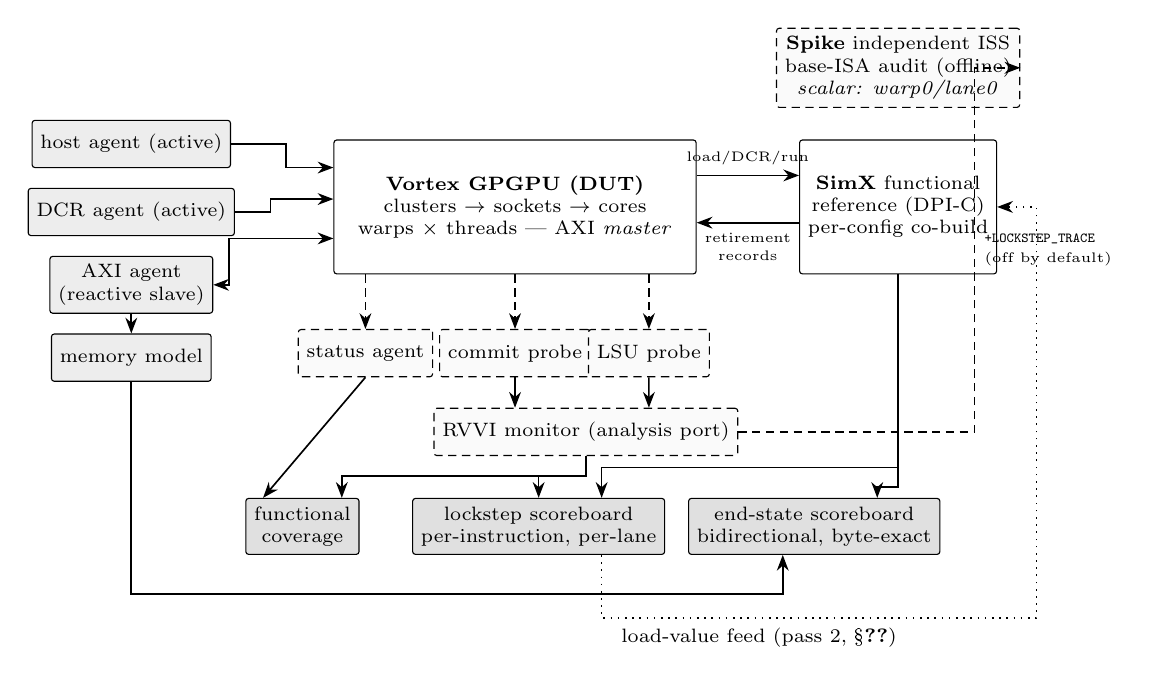
\begin{tikzpicture}[
		font=\scriptsize,
		box/.style={draw, rounded corners=1pt, align=center, inner sep=3pt,
				minimum height=6mm},
		agent/.style={box, fill=gray!14},
		passive/.style={box, fill=gray!4, densely dashed},
		chk/.style={box, fill=gray!24},
		arr/.style={-{Stealth[length=2mm]}, semithick},
		tap/.style={-{Stealth[length=2mm]}, semithick, densely dashed}
		]
		\node[box, minimum width=46mm, minimum height=17mm] (dut)
		{\textbf{Vortex GPGPU (DUT)}\\
			clusters $\to$ sockets $\to$ cores\\
			warps $\times$ threads --- AXI \emph{master}};
		\node[agent, left=13mm of dut.west, anchor=east, yshift=8mm] (host)
		{host agent (active)};
		\node[agent, below=2.5mm of host] (dcr) {DCR agent (active)};
		\node[agent, below=2.5mm of dcr] (axi) {AXI agent\\(reactive slave)};
		\node[agent, below=2.5mm of axi] (mem) {memory model};
		\node[box, right=13mm of dut.east, anchor=west, minimum height=17mm] (simx)
		{\textbf{SimX} functional\\ reference (DPI-C)\\ per-config co-build};
		\node[passive, above=4mm of simx.north, anchor=south, minimum width=30mm] (spike)
		{\textbf{Spike} independent ISS\\ base-ISA audit (offline)\\ \emph{scalar: warp0/lane0}};
		\node[passive] (status) at ($(dut.south)+(-19mm,-10mm)$) {status agent};
		\node[passive] (cprobe) at ($(dut.south)+(0mm,-10mm)$)  {commit probe};
		\node[passive] (lprobe) at ($(dut.south)+(17mm,-10mm)$) {LSU probe};
		\node[passive] (rvvi) at ($(dut.south)+(9mm,-20mm)$)
		{RVVI monitor (analysis port)};
		\node[chk] (cov) at ($(dut.south)+(-27mm,-32mm)$)
		{functional\\ coverage};
		\node[chk] (lss) at ($(dut.south)+(3mm,-32mm)$)
		{lockstep scoreboard\\ per-instruction, per-lane};
		\node[chk] (ess) at ($(dut.south)+(38mm,-32mm)$)
		{end-state scoreboard\\ bidirectional, byte-exact};
		\draw[arr] (host.east) -- ++(7mm,0) |- ([yshift=5mm]dut.west);
		\draw[arr] (dcr.east)  -- ++(4.5mm,0) |- ([yshift=1mm]dut.west);
		\draw[arr, {Stealth[length=2mm]}-{Stealth[length=2mm]}]
		(axi.east) -- ++(2mm,0) |- ([yshift=-4mm]dut.west);
		\draw[arr] (axi) -- (mem);
		\draw[arr] ([yshift=4mm]dut.east) -- ([yshift=4mm]simx.west)
		node[midway, above, font=\tiny] {load/DCR/run};
		\draw[arr] ([yshift=-2mm]simx.west) -- ([yshift=-2mm]dut.east)
		node[midway, below, font=\tiny] {\shortstack{retirement\\records}};
		\draw[tap] ([xshift=-19mm]dut.south) -- (status.north);
		\draw[tap] (dut.south) -- (cprobe.north);
		\draw[tap] ([xshift=17mm]dut.south) -- (lprobe.north);
		\draw[arr] (cprobe.south) -- ([xshift=-9mm]rvvi.north);
		\draw[arr] (lprobe.south) -- ([xshift=8mm]rvvi.north);
		\draw[arr] (rvvi.south) -- ++(0,-2.5mm) -| (lss.north);
		\draw[arr] (rvvi.south) -- ++(0,-2.5mm) -| ([xshift=5mm]cov.north);
		\draw[arr] (status.south) -- ([xshift=-5mm]cov.north);
		\draw[arr] (simx.south) -- ++(0,-27mm) -| ([xshift=8mm]ess.north);
		\draw[arr] (simx.south) -- ++(0,-24.5mm) -| ([xshift=8mm]lss.north);
		\draw[arr] (mem.south) |- ($(ess.south)+(-4mm,-5mm)$)
		-- ($(ess.south)+(-4mm,0)$);
		\draw[arr, dotted] ([xshift=8mm]lss.south) -- ++(0,-8mm)
		-| ($(simx.east)+(5mm,0)$) -- (simx.east);
		\node[below] at ($(lss.south)+(28mm,-8mm)$)
		{load-value feed (pass 2, \S\ref{sec:loadfeed})};
		\draw[tap] (rvvi.east) -- ++(30mm,0) |- (spike.east)
		node[pos=0.25, right, font=\tiny, align=left]
			{\shortstack[l]{\code{+LOCKSTEP_TRACE}\\ (off by default)}};
	\end{tikzpicture}
	\caption{Environment architecture. Solid gray: active UVM agents;
		dashed: passive probes and offline tools; dark: verdict-rendering
		scoreboards and coverage. SimX is the \emph{primary} golden model
		(live over DPI-C, models SIMT, not independent); Spike is a
		\emph{secondary, independent} scalar ISS (offline, base-ISA subset
		only). Neither substitutes for the other.}
	\label{fig:arch}
\end{figure*}

\subsection{Role-inverted agents}
A GPGPU executes programs; it is not driven by them. Five agents
surround the DUT: \emph{host} and \emph{device-configuration-register
	(DCR)} agents (active) drive the launch protocol; the \emph{AXI} agent
is an active \emph{responder}---a reactive slave backed by a memory
model servicing the DUT's fetch and data traffic; a \emph{memory} agent
covers the non-AXI configuration of the same model; a passive
\emph{status} agent observes busy/completion state and retire counts.
Stimulus is a \emph{program} (compiled ELF); the test class controls
only how it is launched, configured, and perturbed.

\subsection{Golden model and probes}
SimX is linked via DPI-C (\code{simx_init}/\code{load}/\code{dcr_write}/%
\code{run} plus per-retirement record export); RTL and SimX are rebuilt
per configuration so DUT and reference always agree on topology.
Golden-model crashes are trapped and mapped to a sentinel exit code, so
a reference failure is \emph{classified}, never a silent pass. All
white-box visibility is bound and passive: a \emph{commit probe} on
every core's retire arbiter capturing
$\{\textit{uuid},\textit{wid},\textit{PC},\textit{rd},\textit{wb},
	\textit{tmask},\textit{per-lane data}\}$; an \emph{LSU writeback probe}
recovering true per-lane load values; an RVVI-style monitor; and
microarchitectural probes (scheduler, divergence/reconvergence,
local-memory bank, coalescer, cache, register-hazard, commit-beat)
feeding the SIMT coverage layer. Lockstep capture is plusarg-gated;
with the gate off, runs are byte-identical to the plain environment.

\subsection{Checkers, configurability, protocol}
Two independent checkers render verdicts: (1)~a \textbf{bidirectional
	end-state scoreboard}---every word the DUT wrote compared byte-exact
against SimX (forward, up to 196{,}868 words in one test) \emph{and}
every word SimX wrote that the DUT never wrote (reverse, catching
dropped stores), with per-byte validity masking and bounded FP
tolerance; (2)~the \textbf{lockstep scoreboard}
(Section~\ref{sec:lockstep}). An assertion gate fails any run with a
firing RTL assertion, excludes it from coverage merging, and is kept
honest by a negative test that must fail through the assertion path
alone. One compiled environment runs any topology from plusargs
(\code{+CLUSTERS}/\code{+CORES}/\code{+WARPS}/\code{+THREADS});
elaboration-time assertions compare every UVM parameter against its DUT
counterpart. An AXI4 SVA layer (${\sim}15$--$18$ properties plus 11
stability assertions) checks burst legality and stability under
backpressure; plusarg-gated \emph{throttle}/\emph{flood} stress modes
and an \emph{error-injection} mode (\code{+AXI_INJECT_ERR}) drive them.

\section{Verdicts and Non-Vacuity}
\label{sec:verdicts}

Every run renders \textsc{pass}, \textsc{fail}, \textsc{unverifiable},
or \textsc{end-state-verified} with an instruction-granularity residual.
\textsc{unverifiable} is first-class: a run the golden model cannot
judge is classified with root cause---never force-compared, never
counted as a pass. Verdicts are only as good as their ability to go
red: every checker is guarded by a permanent fault-injection regression
test---wrong-value (\code{+INJECT_FAULT}) and dropped-store
(\code{+DROP_STORE}) for the end-state scoreboard (both historically
detect at the exact address \code{0x800075d8}); one-bit retirement
corruption (\code{+LOCKSTEP_INJECT}) for the lockstep comparator; and a
RAL mirror corruption (\code{+DCR_RAL_INJECT}) for the register
checker. All must stay red on injection after any checker change---the
mutation-qualification discipline~\cite{vacuity-date10} applied
end-to-end. A nearly-accepted \emph{vacuous} gate pass (negative tests
reporting \textsc{pass} when their injection plusargs were absent) was
caught and codified: always verify the injection message, never the
verdict. This discipline is what allows the coverage and pass-rate
numbers below to be taken at face value.

\section{Per-Instruction Lockstep for SIMT}
\label{sec:lockstep}

The DUT probe stream and the SimX per-retirement stream meet in a
scoreboard that aligns both per (core, warp) and compares each
retirement per active lane (PC, destination, value) with a four-way
outcome taxonomy and drain-empty checks (Fig.~\ref{fig:align}). Five
rules, each forced by simulation evidence and transferable to any SIMT
lockstep, make this sound:

\begin{figure}[t]
	\centering
	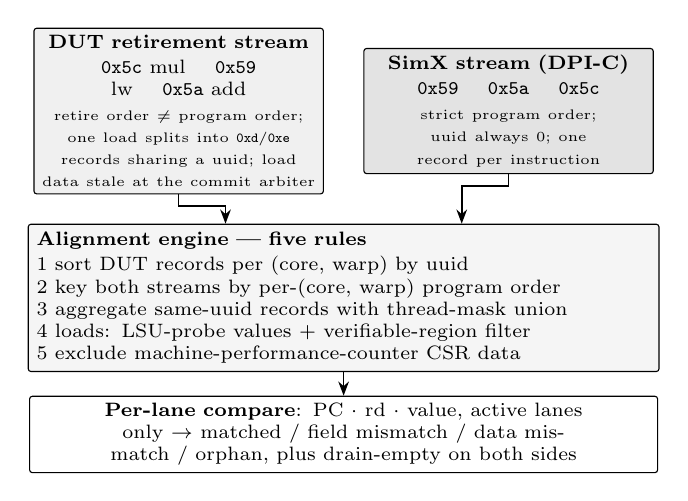
\begin{tikzpicture}[
		font=\scriptsize,
		box/.style={draw, rounded corners=1pt, align=center, inner sep=2.5pt},
		eng/.style={draw, rounded corners=1pt, align=left, inner sep=3pt,
				fill=gray!8},
		arr/.style={-{Stealth[length=1.8mm]}, semithick}
		]
		% two input streams
		\node[box, text width=35mm, fill=gray!12] (dut) at (0,0)
		{\textbf{DUT retirement stream}\\[1pt]
		\code{0x5c} mul \quad \code{0x59} lw \quad \code{0x5a} add\\[1pt]
		{\tiny retire order $\neq$ program order; one load splits into
		\code{0xd}/\code{0xe} records sharing a uuid; load data stale at the
		commit arbiter}};
		\node[box, text width=35mm, fill=gray!22, right=5mm of dut] (simx)
		{\textbf{SimX stream (DPI-C)}\\[1pt]
		\code{0x59} \quad \code{0x5a} \quad \code{0x5c}\\[1pt]
		{\tiny strict program order; uuid always 0; one record per
		instruction}};
		% alignment engine
		\node[eng, below=5mm of $(dut.south)!0.5!(simx.south)$, anchor=north,
			text width=78mm] (engine)
		{\textbf{Alignment engine --- five rules}\\[1pt]
			1~sort DUT records per (core, warp) by uuid\\
			2~key both streams by per-(core, warp) program order\\
			3~aggregate same-uuid records with thread-mask union\\
			4~loads: LSU-probe values + verifiable-region filter\\
			5~exclude machine-performance-counter CSR data};
		% comparator
		\node[box, below=3mm of engine.south, anchor=north, text width=78mm]
		(cmp) {\textbf{Per-lane compare}: PC $\cdot$ rd $\cdot$ value, active
			lanes only $\to$ matched / field mismatch / data mismatch / orphan,
			plus drain-empty on both sides};
		\draw[arr] (dut.south) -- ++(0,-1.5mm)
		-| ([xshift=-15mm]engine.north);
		\draw[arr] (simx.south) -- ++(0,-1.5mm)
		-| ([xshift=15mm]engine.north);
		\draw[arr] (engine.south) -- (cmp.north);
	\end{tikzpicture}
	\caption{The lockstep alignment pipeline. The DUT stream (left) carries
		the SIMT quirks that a scalar-CPU RVVI flow never meets; the reference
		stream (right) is strictly ordered. Each rule removes exactly one class
		of \emph{false} mismatch: sorting fixes out-of-order retirements
		(Rule~1), program-order keying bridges the reference's null uuids
		(Rule~2), mask-union aggregation reassembles split loads (Rule~3), the
		LSU probe with region filter restores sound load comparison (Rule~4),
		and volatile-CSR exclusion removes timing-only divergences (Rule~5).
		After alignment, any remaining difference outside the three declared
		exception classes is a real defect.}
	\label{fig:align}
\end{figure}

\subsubsection{Retire order is not program order} The commit arbiter
retires whichever unit is ready (\code{VX_commit.sv:56-71}); an
earlier-issued instruction was observed retiring after two later ones.
\emph{Align by the per-warp issue counter (uuid), sorted---never by
	position or cycle.}

\subsubsection{The golden model's uuid is not a cross-key} SimX leaves
its uuid at zero. \emph{Align by per-(core, warp) program order; the
	DUT uuid's high bits encode $(\textit{CORE\_ID} \ll \textit{NW\_BITS})
		+ \textit{wid}$ (\code{VX_uuid_gen.sv:40}), supplying attribution with
	no RTL change.}

\subsubsection{One instruction is not one record} A single load appears
as several records sharing one uuid with partial, overlapping masks
(observed \code{0xd} then \code{0xe}) as the LSU commits lanes on
response arrival. \emph{Aggregate DUT records by uuid with thread-mask
	union; never by packet flags.}

\subsubsection{Load data needs its own tap and soundness filter} The
commit arbiter's data field is stale for loads; a dedicated LSU probe
recovers per-lane values, but a naive compare is \emph{unsound} (429
false mismatches on a known-good kernel from uninitialized regions).
\emph{Compare a load lane only when the reference address is in the
	verifiable region and the golden value is not initialization poison;
	defer the rest to end-state.} With the filter, the load compare is
exact (74 compared, 113 filtered, 0 false mismatches).

\subsubsection{Performance-counter CSRs diverge by definition}
\code{mcycle}/\code{minstret}/\code{mhpmcounter*} differ between a
timing-accurate DUT and a functional model (observed off-by-one).
\emph{Flag the MPM CSR range volatile; exclude their data, still check
	PC and destination.}

Beyond the five rules, the comparator declares three bounded, logged
exception classes: the load-value deferral of Rule~4, the volatile-CSR
exclusion of Rule~5, and an \emph{fsqrt-only tolerance}. The DUT's
\code{fsqrt.s} is one ULP off correctly-rounded IEEE~754
(Section~\ref{sec:rtlfindings}), so an \code{fsqrt} writeback is
tolerated iff the two values are same-sign, finite, and within one ULP
(\code{fp32_within_ulp}); every toleranced comparison is tallied
(\code{n_fp_ulp_tol})---logged, never silent. All other floating-point
operations compare bit-exact, and an \code{fsqrt} beyond one ULP, or a
NaN/Inf mismatch, still fails. A two-pass reconvergence feed (armed
with the load feed on \code{+LOCKSTEP_LOADFEED}) then forces the
accepted DUT square-root result into the reference's FP register file
and re-checks every downstream operation bit-exactly, so the accepted
deviation cannot cascade into false errors; the 13-class FPU kernels
verify to residual zero under this handling (1{,}675 matched
retirements). Each rule also carries a DUT precondition an adopter
must re-derive: Rule~1 a unique per-warp issue counter that does not
wrap within a run; Rule~2 a stable (core, warp) attribution key;
Rule~3 records that may split per lane but share an identifier;
Rule~4 a tap where true load values are observable; Rule~5 knowledge
of the model-divergent CSR ranges.

The lockstep was validated lane-exact---0 mismatches, 0 orphans---%
across a configuration matrix spanning
$\textit{NCL}\in\{1,2\}$, $\textit{NC}\in\{1,2\}$,
$\textit{NW}\in\{2,4,8\}$, $\textit{NT}\in\{2,4\}$
(Table~\ref{tab:matrix}), including nested-divergence kernels
($3\text{v}1 \to 2\text{v}1 \to 1\text{v}1$) exercising mask-union
aggregation through divergence and reconvergence with no comparator
changes.

\begin{table}[t]
	\caption{Lockstep configuration matrix (all lane-exact: 0 mismatches,
		0 orphans). Tallies are recorded in the verification documentation;
		per-run raw logs were not retained.}
	\label{tab:matrix}
	\centering
	\small
	\begin{tabular}{lr}
		\toprule
		Configuration                    & Matched writebacks \\
		\midrule
		1CL/1C/4W/4T (vector-add)        & 1{,}035 / 1{,}035  \\
		1CL/1C/4W/4T (nested divergence) & 2{,}668 / 2{,}668  \\
		1CL/2C/4W/4T                     & 1{,}801 / 1{,}801  \\
		2CL/2C/4W/4T                     & 3{,}333 / 3{,}333  \\
		1CL/1C/2W/2T                     & 855 / 855          \\
		1CL/1C/8W/4T                     & 1{,}423 / 1{,}423  \\
		\bottomrule
	\end{tabular}
\end{table}

\section{Verifying Racy Programs: Two-Pass Load-Value Feed}
\label{sec:loadfeed}

Fenceless multi-core programs have no architecturally defined result on
a weakly coherent machine, so per-instruction comparison diverges
legitimately: the two models resolve the same race differently. Rather
than waive such programs, we make them verifiable. Pass~1 records the
DUT's per-lane loaded values at divergent in-region load sites, keyed
by (core, warp, PC, occurrence); pass~2 re-runs the reference following
those values, so the models share the race outcome and the
\emph{residual}, not the feed, is the verdict: a difference not
explained by a fed load stays a hard error. The method rests on an
assumption we state rather than discharge in general---that a divergent
load is a genuine race resolution, not a DUT load-data defect. For the
flagship case this assumption was confirmed by trace analysis: the
first-divergence load reads a word still holding its pristine ELF
initialization value (nothing had overwritten it before the DUT's
read), in a single-hart program running on four shared-memory
cores---a genuine cross-core ordering race. There, 20 racy loads
cascading into 138 divergent retirements collapse to a residual of
\textbf{zero over 5{,}432 retirements}, upgrading the verdict from
\textsc{unverifiable} to \emph{verified modulo the fed race
	resolutions}. The boundary is stated, not hidden:
for an \emph{interrupt} test the feed collapses 116 divergences to 7
but not 0, because the two models take the interrupt at different
instruction boundaries; re-keying the feed leaves the residual
identical, proving it is not an alignment artifact. Interrupt-timing
divergence therefore remains instruction-granularity unverifiable,
while end-state still passes. \emph{Two-pass replay is a fixed point
	for data-only divergence; asynchronous-input timing requires a
	step-follower reference.}

\section{Stimulus}
\label{sec:stimulus}

\textbf{Directed kernels} (${\sim}30$, all byte-exact against the
reference): arithmetic/memory baselines; all 13 FPU classes; tensor
WMMA including multi-warp launches; nested-divergence towers; barriers
under partial masks; \code{wspawn}/\code{tmc} sweeps; MSHR and
memory-pressure stress; a 232\,KB-text kernel; a 256\,KB store stress;
VOTE/SHFL. \textbf{Constrained-random}: a riscv-dv~\cite{riscvdv}
pipeline targeting rv32im with GPU-specific post-processing; two
profiles are excluded as \emph{unimplementable} (unaligned access, no
misaligned support; illegal instruction, no trap architecture), and
jump-stream generation is sanitized to keep riscv-dv's deliberate
JALR-LSB probing away from R1---the deviation is reported, not hidden.
\textbf{simtgen}: an original random C-kernel generator targeting the
microarchitectural axes scalar generators cannot reach, with knobs
derived from the DUT's own configuration space (warp/thread counts,
coalescer window, local-memory bank count, IPDOM stack depth),
informed by the generation-axis taxonomy published by
FuzzGPU~\cite{fuzzgpu} but implemented against our own checking stack;
no third-party code is used. \code{simtgen} implements four axes:
divergence (structured branch trees with controlled split depths),
memory (stride/scatter/bank-hostile patterns), barrier topology
(single-warp barriers, deadlock-safe by construction), and VOTE/SHFL
(all eight intrinsics per program). The barrier and VOTE/SHFL axes
closed no new coverage---their targets (\code{cp_vote_shfl_op} 8/8,
\code{cross_sfu_threads}) were already fully covered by dedicated
directed kernels; their contribution is generator completeness and
seed-diversity robustness evidence, the same category of result as the
riscv-dv seed farm below. A ten-seed sweep across nine riscv-dv
profiles (90
additional distinct programs, content-hash verified, all passing)
produced \emph{no measurable functional-coverage gain} (every category
bit-identical except toggle $+0.06\%$)---a robustness result reported
as such: coverage saturates inside the scalar generator's reach, and
the remaining work is stimulus of a different \emph{kind}.

\section{Coverage Methodology and Results}
\label{sec:coverage}

\subsection{Three layers, never merged}
\textbf{L1 --- ISA} (third-party riscvISACOV): 80 active covergroups
over RV32I/F/M/Zicsr/Zifencei. Sampling \emph{every active lane as a
	hart} (4{,}581 samples) was proven to cover exactly the same bin set as
lane-0-only (1{,}677)---empirical proof that ISA coverage is blind to
the SIMT axis, which is why L2 exists. A closed gap-hunt leaves 78/80
covergroups real and 429/516 target bins hit (83.14\%; 89.28\%
weighted) after register-index exclusions. \textbf{L2 --- SIMT
	microarchitecture} (this work's contribution): probe-sampled
covergroups for warp divergence crossed with IPDOM depth
(\code{divergence_cg}), reconvergence, barrier scope/events,
\code{tmc}/\code{wspawn}, scratchpad bank conflicts
(\code{lmem_bank_cg}), coalescing classes (\code{coalesce_cg}), cache
events, register hazards, and commit-beat shapes. \textbf{L3 ---
	system/protocol}: SVA assertion coverage, AXI transaction space,
DCR/host launch spaces. Layer databases are never blended.

\subsection{Closure discipline}
(1)~\emph{Exclusions are structural, RTL-cited, machine-generated}:
each waiver carries a \code{file:line} citation (e.g., write-response
stability is unreachable because the adapter hardwires
\code{m_axi_bready=1'b1}, \code{VX_axi_adapter.sv:313}), and a blocking
\emph{hits-invariant} merge gate verifies every waived bin had zero
hits unwaived---on first execution it caught two real waiver defects,
one latent for weeks. (2)~\emph{Reachable-but-unhit stays red}:
never waived. (3)~\emph{Ceilings are root-caused}: the toggle plateau
was traced per sub-module to a read-only icache data port (51{,}340
bins, 55.7\% sub-module toggle; 26.4\% of the entire toggle gap from one
subtree, \code{VX_socket.sv:106}) and constant address bits; an
adversarial maximum-entropy kernel moved aggregate toggle $+0.02\%$,
establishing the ceiling as structural. Banks are per-configuration:
cross-topology UCDB merging was shown invalid (instance-set inflation).

\subsection{Results}
Table~\ref{tab:coverage} summarizes the banked configurations.

\begin{table}[t]
	\caption{Coverage banks (QuestaSim; per-configuration, never
		blended). All rows are the 2026-08-16 \emph{pre-relay-fix} banks;
		the reset-fixed 1CL bank (51 runs, 2026-08-18) totals the same
		94.7\% with branch 94.53\% and toggle 83.34\%---indicative only,
		two variables changed (\S\ref{sec:provenance}). A relay-fixed 2CL
		bank taken after this table was frozen (110 runs, 0 failures,
		93.4\% covergroup bins / 94.3\% total, on the grown
		post-remediation coverage model) restores cross-configuration
		comparability; the pre-fix columns are retained for provenance.}
	\label{tab:coverage}
	\centering
	\small
	\setlength{\tabcolsep}{4.5pt}
	\begin{threeparttable}
		\begin{tabular}{lrr}
			\toprule
			Metric                & 1CL/1C/4W/4T       & 2CL/2C/4W/4T      \\
			\midrule
			Covergroup bins (raw) & 370/377 = 98.1\%   & 989/1032 = 95.8\% \\
			Covergroup (weighted) & 99.8\%             & 99.5\%            \\
			Statement             & 98.1\%             & 98.3\%            \\
			Branch                & 95.1\%             & 95.7\%            \\
			Condition             & 90.4\%             & 88.8\%            \\
			Toggle                & 82.8\%             & 80.5\%            \\
			Assertion             & 96.9\%             & 98.9\%            \\
			Directive             & 100.0\%            & 100.0\%           \\
			\midrule
			\textbf{Total}        & \textbf{94.7\%}    & \textbf{94.6\%}   \\
			Runs passing          & 50/50$^{\ddagger}$ & 50/50             \\
			Coverage instances    & 2\,256             & 8\,275            \\
			\bottomrule
		\end{tabular}
		\begin{tablenotes}\footnotesize
			\item[$\ddagger$] \emph{Simulation runs}, not programs: 49
			distinct programs, one run twice under two bus modes.
			\item A third bank with shared L2/L3 enabled totals 93.2\%
			(51 runs, all passing), also on the pre-fix design.
		\end{tablenotes}
	\end{threeparttable}
\end{table}

\subsection{SIMT-layer closures and honesty notes}
Before simtgen, three SIMT targets were open: depth-4 IPDOM divergence
(\code{cp_split_depth} 3/4---depth~3 unhit across 50 seeds), the
bank-conflict bin (\code{lmem_bank_cg} 0/3, never sampled in
70{,}498+ cycles), and one apparent coalescing gap. Deliberate simtgen
programs closed the first two (Fig.~\ref{fig:simtclosure}): depth 4/4
and real bank conflicts surfaced; both closures are folded into a
suite bank (2026-09-09). Three attribution notes travel with this
result, each established by experiment: (a)~the bank-conflict
``gap'' was in fact a \emph{coverage-model defect}: the
coverpoint was defined over \emph{accepted} requests, but the
local-memory crossbar admits exactly one winner per bank per
cycle---``two accepted requests on one bank'' was structurally
impossible, and deliberate bank-hostile stimulus proved it (zero
conflicts); reclassifying onto \emph{offered} requests made the bin
reachable and honest (169 conflict hits), so the closure credit is
shared between the probe fix and the generator;
(b)~the coalescing classes, which an earlier isolated-merge report
attributed to simtgen, were re-examined and found already covered by
the existing coalescer probe and kernels---an attribution correction
we report rather than quietly keep; (c)~the barrier and VOTE/SHFL
generator axes closed nothing because their targets were already fully
covered by directed kernels (above). A
coverage definition must itself be validated against the RTL's
structure; the stimulus gap and the taxonomy defect were disentangled
by experiment. The marginal picture per
generator kind: ninety additional riscv-dv
programs closed zero bins (the seed-farm result), while 57 simtgen
programs (divergence and memory axes) closed the divergence and
bank-conflict targets---stimulus
\emph{kind}, not volume, moves this coverage model.

\begin{figure}[t]
	\centering
	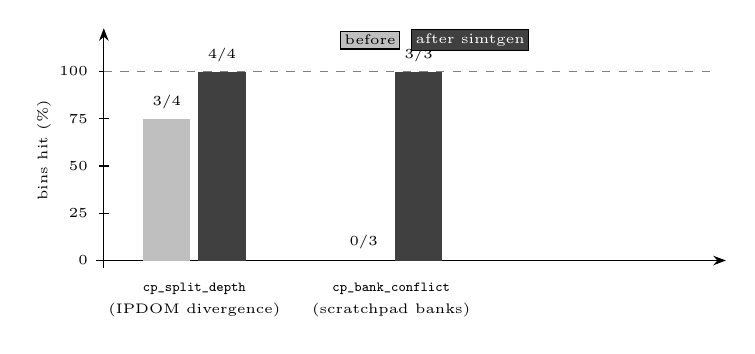
\begin{tikzpicture}[font=\scriptsize]
		% axes
		\draw[-{Stealth[length=1.6mm]}] (-0.1,0) -- (7.9,0);
		\draw[-{Stealth[length=1.6mm]}] (0,-0.1) -- (0,2.95);
		\node[rotate=90, font=\tiny, anchor=south] at (-0.55,1.4) {bins hit (\%)};
		\foreach \y/\l in {0/0, 0.6/25, 1.2/50, 1.8/75, 2.4/100}
			{\draw (-0.06,\y) -- (0.06,\y);
				\node[left] at (-0.08,\y) {\tiny \l};}
		\draw[dashed, gray] (0,2.4) -- (7.7,2.4);
		% cp_split_depth: 3/4 -> 4/4
		\fill[gray!50] (0.5,0) rectangle (1.1,1.8);
		\fill[black!75]  (1.2,0) rectangle (1.8,2.4);
		\node[above] at (0.8,1.8)  {\tiny 3/4};
		\node[above] at (1.5,2.4)  {\tiny 4/4};
		% cp_bank_conflict: 0/3 -> 3/3 (before value is exactly zero: no bar)
		\fill[black!75]  (3.7,0) rectangle (4.3,2.4);
		\node[above] at (3.3,0.02) {\tiny 0/3};
		\node[above] at (4.0,2.4)  {\tiny 3/3};
		% x labels (two groups; the coalescing group was removed after the
		% attribution re-examination: cp_coalesce_kind was already covered
		% by the existing coalescer probe/kernels before simtgen)
		\node[align=center] at (1.15,-0.5) {\tiny \code{cp_split_depth}\\
			\tiny (IPDOM divergence)};
		\node[align=center] at (3.65,-0.5) {\tiny \code{cp_bank_conflict}\\
			\tiny (scratchpad banks)};
		% legend
		\node[draw, fill=gray!50, inner sep=1.5pt, font=\tiny, anchor=west]
		at (3.0,2.8) {before};
		\node[draw, fill=black!75, inner sep=1.5pt, font=\tiny, anchor=west,
			text=white] at (3.9,2.8) {after simtgen};
	\end{tikzpicture}
	\caption{Effect of axis-directed generation on the two SIMT targets
		it genuinely closed (bins hit, as a percentage of the coverpoint's
		bin count). Before simtgen (light bars): depth-4 IPDOM divergence
		was unreachable by any of 50 random-program seeds (3/4 bins); bank
		conflicts never occurred in 70{,}498+ sampled cycles (0/3---itself
		root-caused to a coverpoint-definition defect, since the crossbar
		admits one winner per bank per cycle). Deliberate divergence-tower
		and bank-hostile kernels (dark bars) closed both to 100\%, now
		folded into a suite bank (2026-09-09). A third target previously
		reported here (coalescing classes) was re-examined and found
		already covered by the existing coalescer probe and kernels
		before simtgen existed---an attribution correction to our earlier
		isolated-merge reporting.}
	\label{fig:simtclosure}
\end{figure}

\subsection{Provenance of the DUT}
\label{sec:provenance}
The design is pinned at a specific revision \emph{with eighteen locally
	modified files in the synthesizable RTL tree} (mostly
simulator-compatibility fixes; the environment is new code). We
disclose this because a verification result is a statement about a
specific artifact. One modification's history is instructive: library
counter assertions fired during bring-up and were guarded off (skip on
unknown inputs) so the environment could run---for months. Restoring
the original assertion and root-causing it exposed R10
(Section~\ref{sec:r10}); after the fix, the assertions pass with no
guard and the local modification was retired in favor of the unmodified
upstream file. Fixing the defect \emph{reduced} branch coverage
(95.1\%$\to$94.5\%): modules behind a relay had been executing
normal-operation paths during an unknown-reset cycle, counted as
covered branches. No coverage metric can report that some of its
coverage came from a state that cannot legitimately arise; we report
the lower figure. (Two variables changed; the delta is indicative.)

\section{Findings I: RTL}
\label{sec:rtlfindings}

All findings are maintained in an evidence-cited register (one entry
each: what
was seen, \code{file:line}/run evidence, class, disposition).
Table~\ref{tab:rtlobs} summarizes R1--R10.

\begin{table}[t]
	\caption{RTL findings. The R1 spec deviation was independently found
		by FuzzGPU~\cite{fuzzgpu} in the ISS component (S2, PR~\#339);
		their RTL findings (X1--X3) are disjoint from ours; R2 was
		independently fixed
		upstream.}
	\label{tab:rtlobs}
	\centering
	\scriptsize
	\begin{tabular}{p{0.4cm}p{3.3cm}p{1.7cm}p{1.4cm}}
		\toprule
		ID  & Finding                                                           & Class         & Disposition                         \\
		\midrule
		R1  & JALR LSB not cleared; odd PC propagates via AUIPC                 & Bug (ISA)     & needs RTL fix; stimulus sanitized   \\
		R2  & \code{STALL_TIMEOUT} \code{1**N}$\equiv$1; watchdog never scales  & Bug (latent)  & fixed; independently fixed upstream \\
		R3  & Misaligned access: no trap; silently retargeted/torn              & Hazard        & per SW contract; gated              \\
		R4  & Core self-starts; DCRs unreset                                    & Hazard        & worked around                       \\
		R5  & Per-warp out-of-order commit                                      & Quirk         & handled (\S\ref{sec:lockstep})      \\
		R6  & One load $\to$ multi records, overlapping masks                   & Quirk         & handled (\S\ref{sec:lockstep})      \\
		R7  & uuid encodes flat core+warp id                                    & Quirk         & exploited (\S\ref{sec:lockstep})    \\
		R8  & Load data unobservable at commit arbiter                          & Observability & closed (LSU probe)                  \\
		R9  & Fire-and-forget writes; \emph{no AXI error path}                  & Characteriz.  & cited; fault-injected (166)         \\
		R10 & Reset relay: reset registered in an unreset flop; X for one cycle & Bug (X)       & fixed; still upstream               \\
		\bottomrule
	\end{tabular}
\end{table}

\subsection{Unknown reset for one cycle, found by restoring a silenced
	assertion (R10)}
\label{sec:r10}
Reset is distributed through a relay that registers it in a flip-flop
nothing resets:

\begin{lstlisting}
`PRESERVE_NET reg [R-1:0] reset_r;   // no initial value
always @(posedge clk) reset_r[i] <= reset;
assign reset_o[i] = reset_r[i / F]; // X until first edge
\end{lstlisting}

Every module behind a relay observes an unknown reset for one cycle;
\code{if (X)} takes the non-reset branch, so reset-held logic executes
and assertions evaluate on unknown operands. The counter assertions
that first flagged this had been \emph{guarded off for months}; the
assertion had been correct the entire time---what was suppressed was
the report, not the problem. We replaced the relay with an
async-assert/sync-deassert synchronizer: twelve firings become zero
with the upstream file unmodified, a 51-run regression passes with
assertions armed, and the injection guards were re-confirmed. The
defect remains in the current upstream release. Two generalizations:
\textbf{a checker disabled to make a bench run is a checker whose
	findings are lost---silently and open-endedly}; and \textbf{fixing a
	defect can reduce a coverage number} (Section~\ref{sec:provenance}).

\subsection{JALR does not clear the target LSB (R1)}
The RISC-V specification~\cite{riscv-spec} requires JALR to clear the
target LSB. Vortex omits the clear (\code{VX_alu_int.sv:222}), and with
no trap architecture cannot raise the prescribed misaligned-target
exception. In the debug build (\code{PC_BITS=XLEN}) the odd bit
survives as the \emph{architectural} PC: fetch silently word-aligns, so
execution continues correctly, but \code{auipc}/\code{la} inherit the
skew, link registers accumulate it across chained jumps ($+1 \to +3$
observed), and downstream accesses go misaligned (R3). The trigger is
spec-legal: riscv-dv deliberately sets the JALR base LSB expecting the
clear, so roughly half of generated jumps derail---every profile of a
12-profile suite fired misaligned assertions (30--7{,}616 per run). The
release build is spec-correct \emph{by accident} (PC bits masked).
FuzzGPU~\cite{fuzzgpu} found the same deviation independently from an
entirely different flow (S2, upstream PR~\#339---filed against the
project's instruction-set simulator; their RTL findings X1--X3, at a
different pin, are disjoint from ours)---independent corroboration of
the \emph{deviation}, though not of its RTL embodiment.

\subsection{Further verified defects}
\textbf{fsqrt.s one ULP off correctly-rounded IEEE~754~\cite{ieee754}}:
a
lockstep lane-0 mismatch (DUT \code{0x3fef7750} vs.\ reference
\code{0x3fef7751}) localized to the sqrt unit; the end-state FP
tolerance absorbs it---\emph{only} per-instruction comparison surfaces
it. \textbf{Memory-scheduler timeout misdenominated}: beside
R2, a picoseconds-denominated localparam yields ${\sim}1{,}000$-cycle
watchdogs, flooding L2/L3 runs with 22{,}187 false alarms while
functionally clean. \textbf{No AXI error path} (R9): the
adapter hard-asserts \code{OKAY}; injecting \code{SLVERR}/\code{DECERR}
every 7th transaction produced 166/166 assertion firings and no
recovery path---an evidence-based upgrade of a waiver into a measured
design limitation.

\section{Findings II: Reference Model}
\label{sec:reffindings}

\emph{A lockstep flow verifies the reference model as much as the
	DUT.} SimX read instructions at the exact byte PC; a computed jump to
an odd target (tolerated by the RTL, which word-aligns) made the
reference read across an instruction boundary and abort, silently
classifying runs unverifiable. The lockstep's divergence report
localized it; word-aligning the reference fetch recovered the runs. The
\emph{obvious} fix---masking the JALR target in the model---was tried
and \emph{reverted with evidence}: 21{,}968 phantom mismatches, because
it fixed the model to the specification rather than the DUT. Further:
SimX aborts on unknown input at 56 disassembly-verified sites (35
decode, 21 execute), mostly in the pretty-printer---a run can be
unverifiable because the golden model could not \emph{name} an
instruction; lockstep upgrades such verdicts to ``byte-exact for all
17{,}664 retirements before abort.'' A SIMT-divergent CSR access
produced 109 genuine mismatches (reference serialized lanes over the
per-warp \code{fcsr}; RTL reads-broadcast/writes lane~0)---the model
was corrected; the RTL quirk is documented, not mirrored.

\section{Limitations and Soundness Boundary}
\label{sec:limits}
\begin{itemize}
	\item \textbf{Asynchronous interrupt timing}: the interrupt test
	      collapses 116$\to$7 but not 0; the residual is keying-independent and
	      genuine (Section~\ref{sec:loadfeed})---end-state \textsc{verified},
	      instruction-granularity residual classified, not forced green.
	\item \textbf{Control-flow-steering races}: when racy loads feed
	      branches, pass-2 replay meets fresh unkeyed races (residual 15,
	      thirteen of them load-class); no fixed point exists---left honestly
	      red.
	\item \textbf{Structural blindness of differential testing}: DUT and
	      reference execute the same binary, so a stimulus fault (e.g., a kernel
	      whose compile-time geometry mismatches the RTL configuration) is
	      invisible---both models wrong identically while every checker passes;
	      equivalence validates only what \emph{differs}; shared inputs need
	      independent assertions. We closed exactly one such input and report
	      the class open.
	\item \textbf{No independent SIMT reference}---structural ceiling, not
	      unfinished task.
	\item \textbf{D-extension elaboration, scoped by inspection}: the
	      primary configuration
	      elaborates the D extension and MISA reports D=1 (\code{FLEN=64},
	      confirmed by elaboration probe) although the toolchain builds RV32IMAF
	      and the reference models F only---unintentional-by-documentation as an
	      RTL fact. Its coverage impact is bounded by code inspection and
	      confirmed by an EXT\_D-off recompile bin diff: zero scored bins
	      change (delta confined to two weight-0 coverpoints). The
	      coverage model's only D-specific bin (float--double conversion) is
	      config-aware-excluded at RV32 (\code{ignore\_bins}), the ISA layer
	      compiles no D plan, and no stimulus can emit a D operation---so no
	      functional bin is diluted. The elaborated-but-unexecuted D logic sits
	      only in code-coverage denominators, which makes the reported totals
	      \emph{conservative} (they understate an F-only build), never inflated.
	\item \textbf{Per-mnemonic aliasing}: the frozen banks predate
	      discovery that instruction-class encodings alias (\code{4'b1011} is
	      both a zero-conditional op and \code{EBREAK}); per-mnemonic claims use
	      only post-remediation measurements.
	\item \textbf{Generality}: all results are one DUT, one simulator, one
	      build; the alignment rules' DUT preconditions are stated in
	      Section~\ref{sec:lockstep}, and transfer beyond them is belief, not
	      demonstration.
	\item \textbf{Scope}: this is front-end RTL functional
	      verification---gate-level, timing, DFT, CDC, and physical sign-off are
	      prerequisites for a different claim entirely and are out of scope.
\end{itemize}

\section{Conclusion}
\label{sec:conclusion}
We presented a UVM environment and closure methodology that brings
reference-model verification
to a SIMT GPGPU, with the first published SIMT functional-coverage
layer for RTL GPU verification. Five alignment rules, each with a
stated DUT precondition, make
per-instruction lockstep sound for SIMT; a two-pass load feed verifies
racy programs at instruction granularity (residual 0 over 5{,}432
retirements, verified modulo the fed race resolutions) with an honestly
characterized boundary; the closure methodology---machine-generated,
gate-checked exclusions, root-caused ceilings, residual bins
dispositioned rather than waived---carried the primary configuration
to 98.1\%/94.7\%; and
every verdict is backed by injection-proven checkers. The checking
depth paid for itself on both sides of the comparison---an externally
corroborated ISA deviation, an upstream-fixed watchdog defect, a
reset-relay X window found by unsuppressing an assertion, and a
reference-model fetch bug found by the lockstep itself. The central
lesson---the reference model must be verified alongside the DUT, and
the coverage model alongside both---transfers to other open SIMT
designs and fills the half of the open-GPU verification problem that
fuzzing does not address.

\balance
\begin{thebibliography}{20}

	\bibitem{vortex-micro}
	B.~Tine, K.~P. Yalamarthy, F.~Elsabbagh, and H.~Kim,
	``Vortex: Extending the RISC-V ISA for GPGPU and 3D-graphics,''
	in \emph{Proc. 54th IEEE/ACM Int. Symp. Microarchitecture (MICRO-54)},
	2021, pp. 754--766.

	\bibitem{vortex-carrv}
	F.~Elsabbagh \emph{et al.},
	``Vortex: OpenCL compatible RISC-V GPGPU,''
	in \emph{Workshop on Computer Architecture Research with RISC-V
		(CARRV)}, 2019.

	\bibitem{fuzzgpu}
	Z.~Gao, J.~Wang, Q.~Zhou, L.~Shan, J.~Hu, X.~Jia, and Z.~Lv,
	``Fuzzing open-source GPU hardware with SIMT program generation,''
	in \emph{Proc. 35th USENIX Security Symposium (USENIX Security~'26)},
	Baltimore, MD, Aug. 2026, pp. 2465--2484.

	\bibitem{difftest}
	Y.~Xu \emph{et al.},
	``Towards developing high-performance RISC-V processors using agile
	methodology,'' in \emph{Proc. 55th IEEE/ACM Int. Symp.
		Microarchitecture (MICRO-55)}, 2022.

	\bibitem{corevverif}
	OpenHW Group, ``core-v-verif: functional verification project for the
	CORE-V family of RISC-V cores,'' [Online]. Available:
	\url{https://github.com/openhwgroup/core-v-verif}

	\bibitem{rvvi}
	OpenHW Group / Imperas, ``RVVI: RISC-V Verification Interface,''
	[Online]. Available: \url{https://github.com/riscv-verification/RVVI}

	\bibitem{riscvdv}
	CHIPS Alliance, ``riscv-dv: SV/UVM based instruction generator for
	RISC-V processor verification,'' [Online]. Available:
	\url{https://github.com/chipsalliance/riscv-dv}

	\bibitem{spike}
	RISC-V International, ``Spike, the RISC-V ISA simulator,'' [Online].
	Available: \url{https://github.com/riscv-software-src/riscv-isa-sim}

	\bibitem{imperasdv}
	Imperas Software, ``ImperasDV: processor verification IP with
	lock-step compare,'' [Online]. Available:
	\url{https://imperas.com/imperasdv}

	\bibitem{uvm}
	\emph{IEEE Standard for Universal Verification Methodology Language
		Reference Manual}, IEEE Std 1800.2-2020, 2020.

	\bibitem{riscv-spec}
	A.~Waterman and K.~Asanovi\'c, Eds., \emph{The RISC-V Instruction Set
		Manual, Volume I: Unprivileged Architecture}, RISC-V Foundation, 2019.

	\bibitem{ieee754}
	\emph{IEEE Standard for Floating-Point Arithmetic}, IEEE Std
	754-2019, 2019.

	\bibitem{gpuverify}
	A.~Betts, N.~Chong, A.~F. Donaldson, S.~Qadeer, and P.~Thomson,
	``The design and implementation of a verification technique for GPU
	kernels,'' \emph{ACM Trans. Program. Lang. Syst.}, vol. 37, no. 3,
	pp. 10:1--10:49, 2015.

	\bibitem{gklee}
	G.~Li, P.~Gopalakrishnan, I.~Ghosh, S.~P. Rajan, and G.~Gopalakrishnan,
	``GKLEE: Concolic verification and test generation for GPUs,''
	in \emph{Proc. ACM SIGPLAN Symp. Principles and Practice of Parallel
		Programming (PPoPP)}, 2012, pp. 215--224.

	\bibitem{deepsmith}
	C.~Cummins, P.~Petoumenos, H.~Leather, and S.~Fursin,
	``Compiler fuzzing through deep learning,'' in \emph{Proc. ACM
		SIGSOFT Int. Symp. Software Testing and Analysis (ISSTA)}, 2018,
	pp. 95--105.

	\bibitem{vacuity-date10}
	L.~Di Guglielmo, F.~Fummi, and G.~Pravadelli,
	``Vacuity analysis for property qualification by mutation of
	checkers,'' in \emph{Proc. Design, Automation \& Test in Europe
		(DATE)}, 2010, pp. 262--267.

	\bibitem{nvbitfi}
	T.-T.~Tsai, S.~K.~S. Hari, M.~Sullivan, O.~Villa, M.~B. Glick, and
	S.~W. Keckler, ``NVBitFI: Dynamic fault injection methodology for GPU
	applications,'' in \emph{Proc. IEEE/IFIP Int. Conf. Dependable Systems
		and Networks (DSN)}, 2021, pp. 64--76.

	\bibitem{rtlcheck}
	Y.~A. Manerkar, D.~Lustig, M. Martonosi, and M. Pellauer,
	``RTLCheck: A property checking approach for custom memory consistency
	models,'' in \emph{Proc. 50th IEEE/ACM Int. Symp. Microarchitecture
		(MICRO-50)}, 2017, pp. 713--725.

	\bibitem{ptxmem}
	D.~Lustig, S.~Sahasrabuddhe, and M.~Giroux,
	``A formal analysis of the NVIDIA PTX memory model,'' in \emph{Proc.
		Int. Conf. Architectural Support for Programming Languages and
		Operating Systems (ASPLOS)}, 2019, pp. 253--266.

	\bibitem{opentitan}
	lowRISC, ``OpenTitan: open source silicon root of trust,'' [Online].
	Available: \url{https://github.com/lowRISC/opentitan}

\end{thebibliography}

\end{document}
